\subsection{Grip force} % \label{app:...}

This test uses the test setup seen on \figref{fig:one_clamp}. The positive force is defined as downwards direction on the load-cell, see \figref{fig:mes_up_down1}.

\begin{figure}[H]
	\centering
	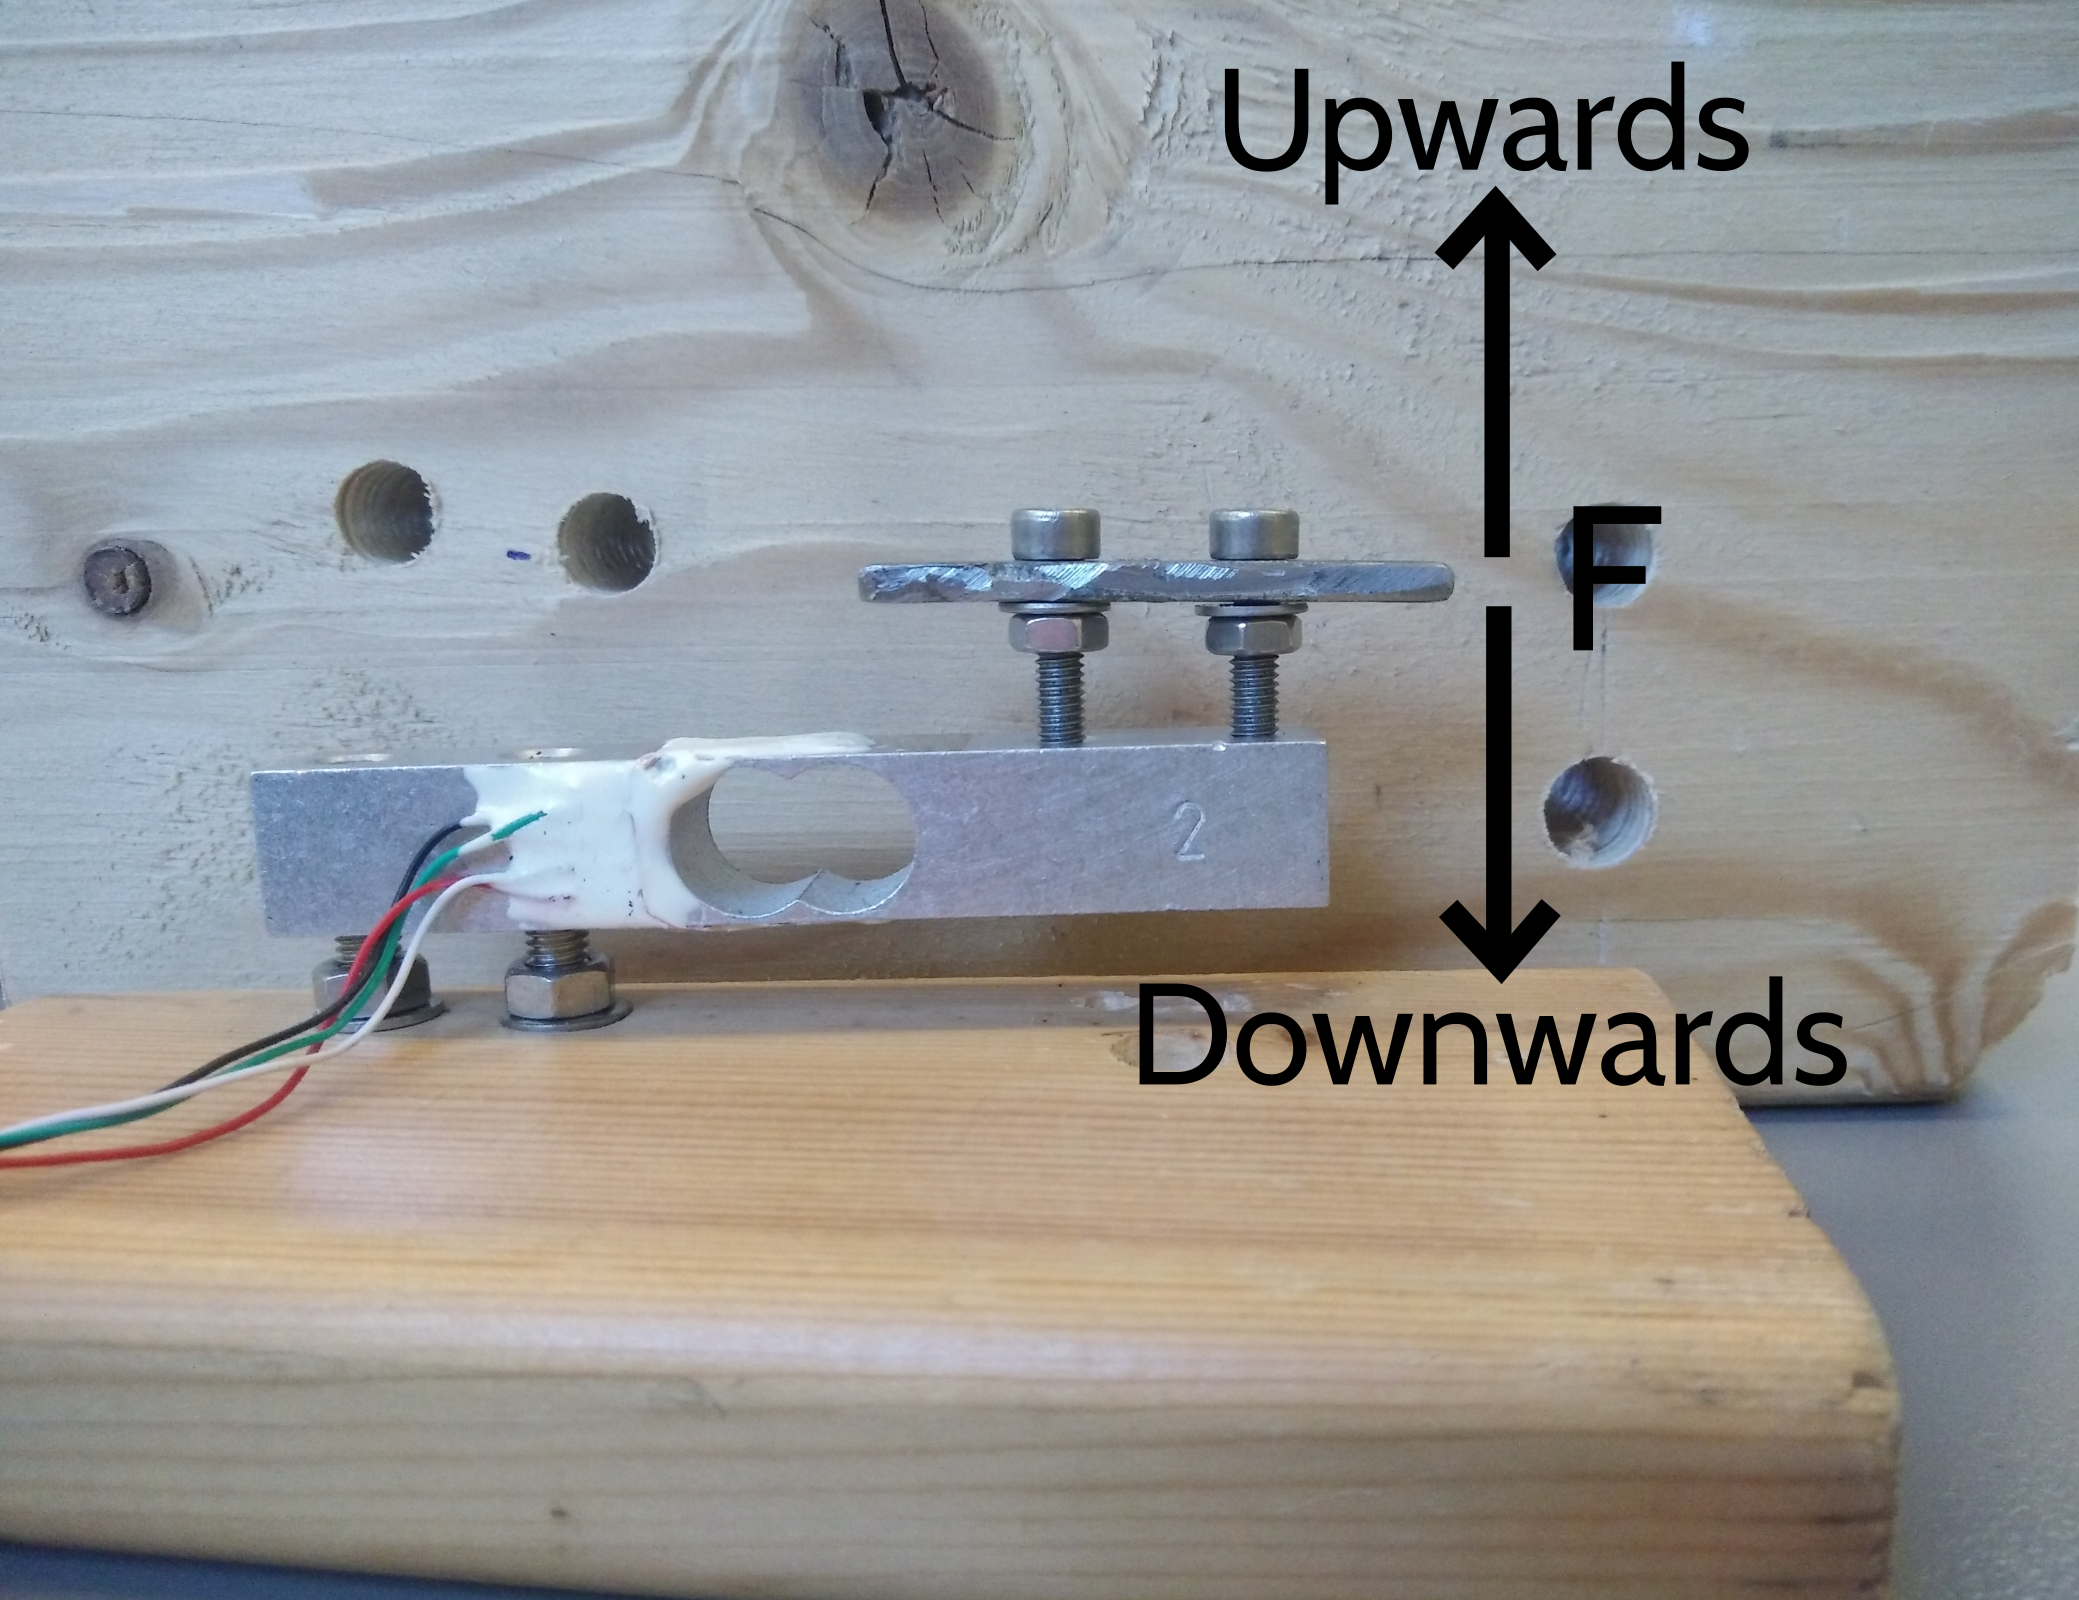
\includegraphics[width=0.4\linewidth]{load_cell_mes.png}
	\caption{Load-cell with defined upwards- downwars force.}
	\label{fig:mes_up_down1}
\end{figure}


\subsection*{Test equipment:}
\begin{itemize}
\item Endowrist model 420093 (AAU number: \#4).
\item Maxon 110160 motor with attached Maxon gearhead 110356 and Maxon encoder 201937.
\item Load cell rate for 1 kg of force \cite{Load_cell_1kg}.
\item HX711 - Load cell amplifier \cite{HX711}.
\item Arduino uno with Max351 DAC.
\item sbRIO board.
\end{itemize}

\subsection*{Procedure:}
The following procedures was made for the dynamic measurements of one clamp on the EndoWrist.

\begin{enumerate}
\item One clamp is enabled and put above the load-cell as seen on \figref{fig:one_clamp}.
\item The scale is set to zero.
\item Alternating setpoints are send to the motor controlling the upper clamp in a triangular wave.
\item Current, force and velocity is sampled.
\end{enumerate}
Each test is running for a short period of time, since the input setpoints are periodic. This test was done 11 times.

\subsection*{Measuring data:}
The data form one measurement is shown on \figref{yaw_mes123}.
\begin{figure}[H]
\centering
\input{Data/Measurement/EndoWrist_Measurements/Force/yaw_mes}
\caption{One set of data that shows the force, current and velocity. The interval between the red lines shows one period of contact with the load cell and the green is the release of the force applied.}
\label{yaw_mes123}
\end{figure}

%\figref{endo_force_mes}. 
%\eqref{eq:linear_force_endo}.

% \begin{equation}
% \text{y} = 0.0028 \cdot \text{x} -0.8259 
% \label{eq:linear_force_endo}
% \end{equation} 


\subsection*{Results:}
From \figref{yaw_mes123}, one of the measurements for the grip force estimation is shown. The first red line marks one of the starting periods, where contact between the clamp and the load-cell is happening. It can be seen that a current increase is happening in when the load-cell is applied force. When the current decreases the force is kept until the sign on the current has changed and force is applied in an upwards direction of the clamp. 


%It can be seen from the graph on \figref{endo_force_mes} that the force on the end-effector is highly nonlinear. The friction from the gearing and the Endowrist does that the force first has an exponential growth at the start. Around the 800 mA and 1200 mA step it can be seen that a drop in force is happening. What causes this drop is not identified but it can be seen that it appears for all the data sequences. \todor{better explanation?}


%% This file was created by matlab2tikz.
%
%The latest updates can be retrieved from
%  http://www.mathworks.com/matlabcentral/fileexchange/22022-matlab2tikz-matlab2tikz
%where you can also make suggestions and rate matlab2tikz.
%
\definecolor{mycolor1}{rgb}{0.00000,0.44700,0.74100}%
\definecolor{mycolor2}{rgb}{0.85000,0.32500,0.09800}%
%
\begin{figure}[h]
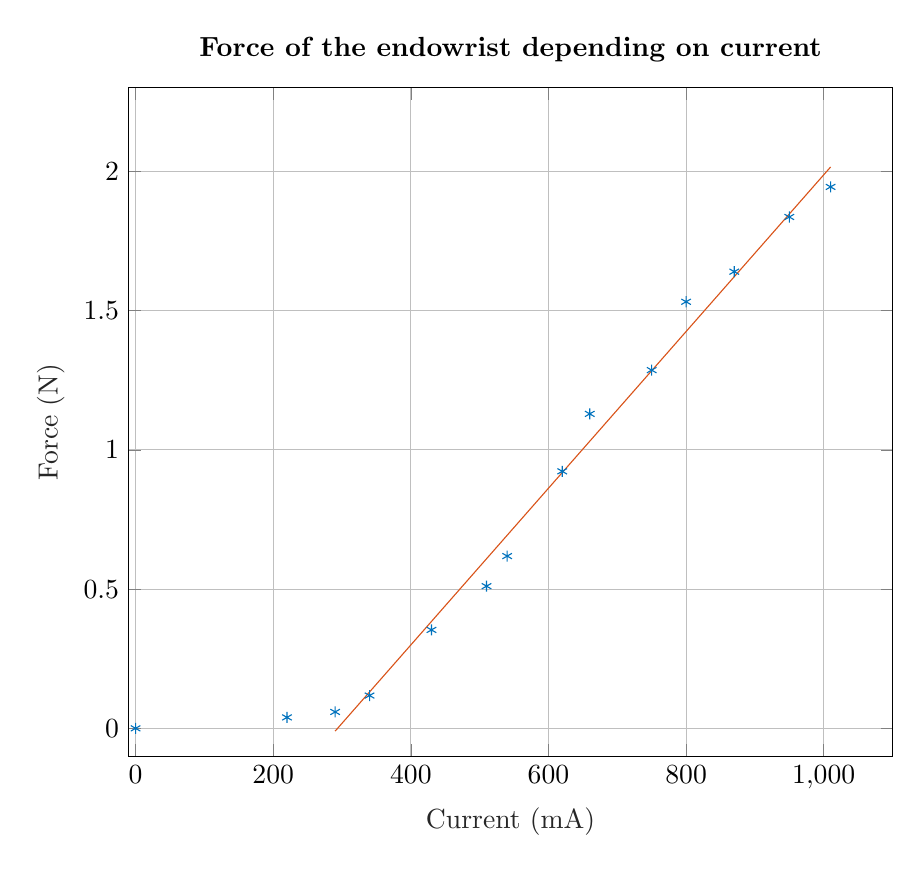
\begin{tikzpicture}

\begin{axis}[%
width=0.8\columnwidth,%7.484in,
height=0.7\columnwidth,%8.26in,
at={(0.758in,0.481in)},
scale only axis,
xmin=-10,
xmax=1100,
xlabel style={font=\color{white!15!black}},
xlabel={Current (mA)},
ymin=-0.1,
ymax=2.3,
ylabel style={font=\color{white!15!black}},
ylabel={Force (N)},
axis background/.style={fill=white},
title style={font=\bfseries},
title={Force of the endowrist depending on current},
xmajorgrids,
ymajorgrids
]
\addplot [color=mycolor1, draw=none, mark=asterisk, mark options={solid, mycolor1}, forget plot]
  table[row sep=crcr]{%
0	0\\
220	0.03928\\
290	0.05892\\
340	0.11784\\
430	0.35352\\
510	0.51064\\
540	0.61866\\
620	0.92308\\
660	1.1293\\
750	1.28642\\
800	1.53192\\
870	1.63994\\
950	1.83634\\
1010	1.94436\\
};
\addplot [color=mycolor2, forget plot]
  table[row sep=crcr]{%
290	-0.00996204344902341\\
340	0.130719594329395\\
430	0.383946542330548\\
510	0.609037162776017\\
540	0.693446145443068\\
620	0.918536765888537\\
660	1.03108207611127\\
750	1.28430902411242\\
800	1.42499066189084\\
870	1.62194495478063\\
950	1.8470355752261\\
1010	2.0158535405602\\
};
\end{axis}
\end{tikzpicture}%
\caption{The force measurements from the end-effector}
\label{endo_force_mes}
\end{figure}

\subsection*{Uncertainties of measurement:}
\begin{itemize}
\item Not 100 \% orthogonal force to the load cell.
\item Input/Output impedance of sensors have a $\pm 10 \%$ tolerance.
\item Movement of test setup when force is generated.
\item The pitch joint of the EndoWrist had a tendency to bend when high force was applied which change the force direction. 
\end{itemize}

\subsection*{Conclusion:}
It can be seen that there is a high friction in mechanical part that handles the clamp. Due to this friction, the tool is able to withhold a force when the current is decreasing.